% 2p5d-two-die: heat-flow network (TikZ).
% Source: config/thermal/2p5d-two-die.yaml (schema v1).
% Compile: pdflatex 2p5d-two-die.tex   (TeX Live 2026; standalone class)
%
% Edge styling: face_adjacency = solid blue (undirected, interposer
% lateral adjacency); vertical_chain = solid amber arrow (lumped R_vert
% to boundary). Reserved types: tsv = dashed, hybrid = dash-dot,
% ground = double (same color families).
\documentclass[border=10pt]{standalone}
\usepackage{sfmath}
\renewcommand{\familydefault}{\sfdefault}
\usepackage{tikz}
\usetikzlibrary{arrows.meta, shapes.geometric}
\definecolor{diefill}{HTML}{E8F0FE}   % die: light blue fill
\definecolor{dieedge}{HTML}{1A73E8}
\definecolor{bndfill}{HTML}{F1F3F4}   % boundary: light gray ellipse
\definecolor{bndedge}{HTML}{5F6368}
\definecolor{faedge}{HTML}{1A73E8}    % face_adjacency: solid blue
\definecolor{vcedge}{HTML}{B45309}    % vertical_chain: solid amber arrow
\begin{document}
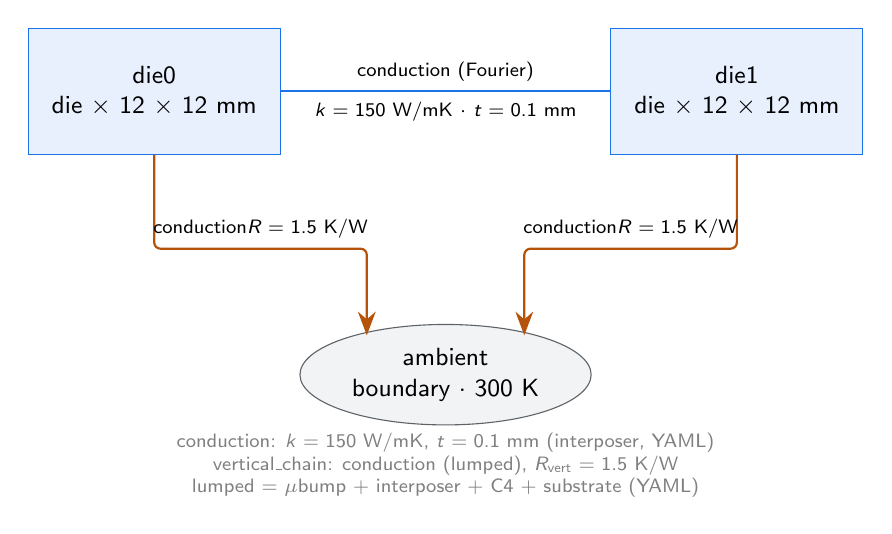
\begin{tikzpicture}[
  die/.style={rectangle, draw=dieedge, fill=diefill, minimum width=3.2cm,
              minimum height=1.6cm, align=center, font=\small},
  bnd/.style={ellipse, draw=bndedge, fill=bndfill, minimum width=3.0cm,
              minimum height=1.1cm, align=center, font=\small},
  fa/.style={draw=faedge, thick},
  vc/.style={draw=vcedge, thick, -{Stealth[length=3mm]}, rounded corners=0.08cm},
  lab/.style={font=\scriptsize},
]
\node[die] (die0) at (-3.7, 0) {die0\\die $\times$ 12 $\times$ 12 mm};
\node[die] (die1) at ( 3.7, 0) {die1\\die $\times$ 12 $\times$ 12 mm};
\node[bnd] (ambient) at (0, -3.6) {ambient\\boundary $\cdot$ 300 K};
\draw[fa] (die0.east) -- node[above, lab] {conduction (Fourier)}
                      node[below, lab] {$k=150$ W/mK $\cdot$ $t=0.1$ mm} (die1.west);
\draw[vc] (die0.south) -- (-3.7,-2.0) -- node[above, lab] {conduction\\$R=1.5$ K/W} (-1.0,-2.0) -- (-1.0,-3.10);
\draw[vc] (die1.south) -- ( 3.7,-2.0) -- node[above, lab] {conduction\\$R=1.5$ K/W} ( 1.0,-2.0) -- ( 1.0,-3.10);
% branch annotation: physical path type + value provenance (geometry+material)
\node[lab, align=center, text=gray] at (0, -4.75) {
  conduction: $k=150$ W/mK, $t=0.1$ mm (interposer, YAML)\\
  vertical\_chain: conduction (lumped), $R_{\mathrm{vert}}=1.5$ K/W\\
  lumped = $\mu$bump + interposer + C4 + substrate (YAML)};
\end{tikzpicture}
\end{document}
